\begin{mainquestion}{nodalpower}{Nodal Analysis II}

\questionpoints Consider the following circuit.

\begin{center}
    % [width=0.8\textwidth] makes the image take up 80% of the text width
    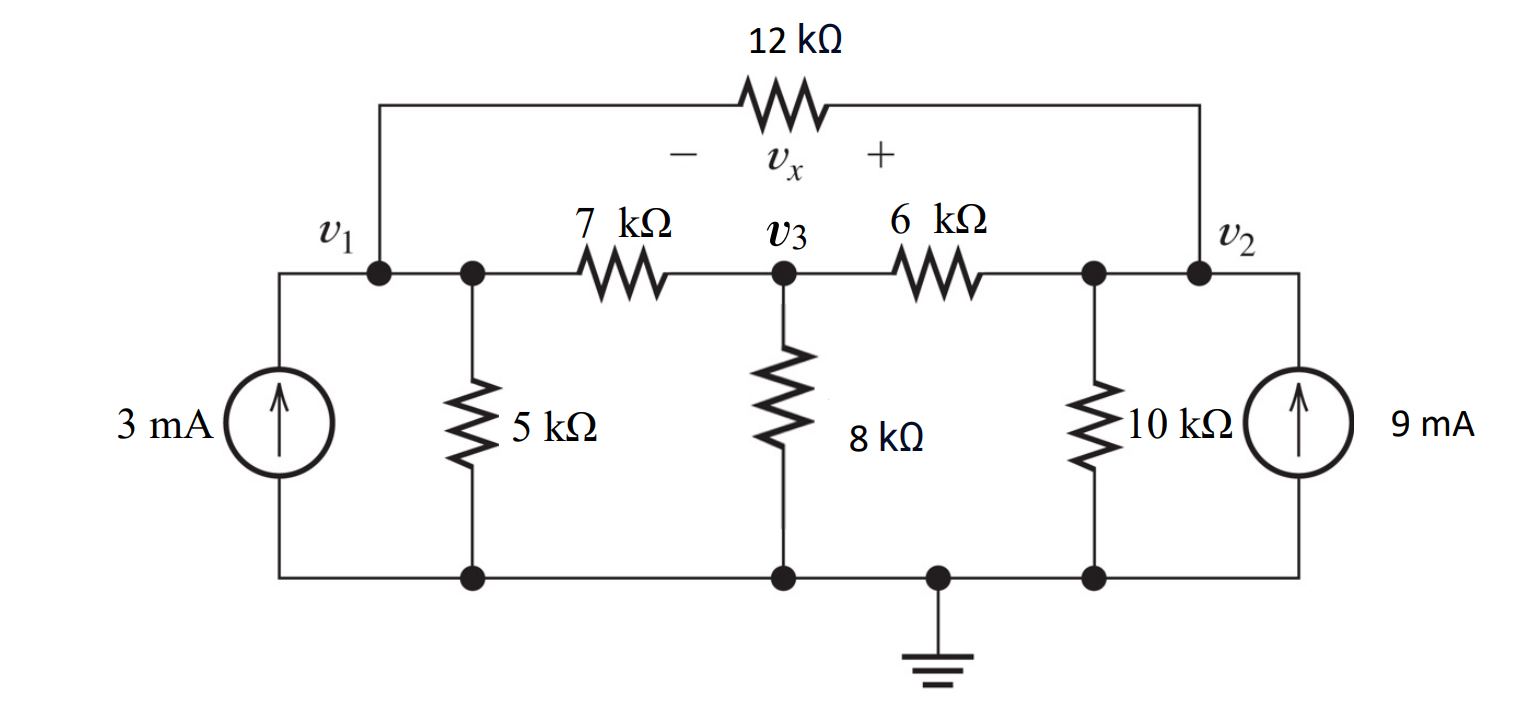
\includegraphics[width=0.8\textwidth]{another_nodal.png}
\end{center}

% =========================================================
\begin{partquestion}{nodal}
{Use nodal analysis to find each of the node voltages $v_{1}, v_{2}$ and $v_{3}$.}

\begin{answer}[4in]
\end{answer}

\end{partquestion}

% =========================================================
\begin{partquestion}{findx}
{Find $v_{x}$.}

\begin{answer}[3in]
\end{answer}

\end{partquestion}

% =========================================================
\begin{partquestion}{branch}
{Find the 8 branch currents $i_{k}$, where $k$ takes on values 1 through 8 (ordered by element position in circuit, from top to bottom, left to right).}

\begin{answer}[4in]
\end{answer}

    \pagebreak
\end{partquestion}

% =========================================================
\begin{partquestion}{power}
{What is the power dissipated in the circuit?}

\begin{answer}[3in]
\end{answer}

\end{partquestion}

% =========================================================
\begin{partquestion}{tellegen}
{What is the total power in the circuit?}

\begin{answer}[1in]
\end{answer}

\end{partquestion}

\end{mainquestion}
